\documentclass{standalone}
\usepackage{tikz}
\usepackage{graphicx} % For rotatebox
\usetikzlibrary{circuits.ee.IEC}

\begin{document}
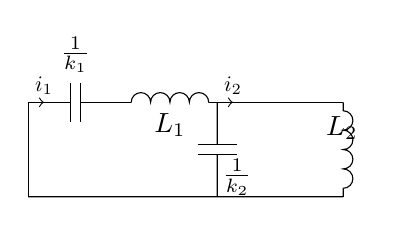
\begin{tikzpicture}[circuit ee IEC, scale=0.8, transform shape]

% Define components
\def\kone{2} % Capacitance 1/k1
\def\ktwo{3} % Capacitance 1/k2
\def\lone{1.5} % Inductance L1

% Draw parallel combination
\draw[fill=gray!30] (0,0) to [capacitor={info={$\frac{1}{k_1}$}}] ++(1.5,0) coordinate (C1)
            to [inductor={info'={$L_1$}, swap}] ++(1.5,0) coordinate (L1);

% Add parallel combination with L2 and 1/k2
\draw[fill=gray!30] (C1) ++(1.5,0) to [capacitor={info={\rotatebox{90}{$\frac{1}{k_2}$}}}] ++(0,-1.5) coordinate (C2);
\draw[fill=gray!30] (C2) ++(2,1.5) to [inductor={info'={\rotatebox{90}{$L_2$}}, swap}] ++(0,-1.5) coordinate (L2);

% Join L1 and L2 with a solid line
\draw (0,-1.5) -- (L2);
\draw (0,0) -- (0,-1.5);
\draw (3,0) --(5,0);

% Add pointer and label for i1
\draw[postaction={decorate,decoration={markings,mark=at position 0.5 with {\arrow{>}}}}] (0,0) -- node[above] {\(i_1\)} (0.5,0);

% Add pointer and label for i2
\draw[postaction={decorate,decoration={markings,mark=at position 0.5 with {\arrow{>}}}}] (3,0) -- node[above] {\(i_2\)} (3.5,0);

\end{tikzpicture}
\end{document}

